% Options for packages loaded elsewhere
\PassOptionsToPackage{unicode}{hyperref}
\PassOptionsToPackage{hyphens}{url}
%


\PassOptionsToPackage{table}{xcolor}

\documentclass[
  10pt,
  letterpaper,
]{article}

\usepackage{amsmath,amssymb}
\usepackage{iftex}
\ifPDFTeX
  \usepackage[T1]{fontenc}
  \usepackage[utf8]{inputenc}
  \usepackage{textcomp} % provide euro and other symbols
\else % if luatex or xetex
  \usepackage{unicode-math}
  \defaultfontfeatures{Scale=MatchLowercase}
  \defaultfontfeatures[\rmfamily]{Ligatures=TeX,Scale=1}
\fi
\usepackage{lmodern}
\ifPDFTeX\else  
    % xetex/luatex font selection
\fi
% Use upquote if available, for straight quotes in verbatim environments
\IfFileExists{upquote.sty}{\usepackage{upquote}}{}
\IfFileExists{microtype.sty}{% use microtype if available
  \usepackage[]{microtype}
  \UseMicrotypeSet[protrusion]{basicmath} % disable protrusion for tt fonts
}{}
\makeatletter
\@ifundefined{KOMAClassName}{% if non-KOMA class
  \IfFileExists{parskip.sty}{%
    \usepackage{parskip}
  }{% else
    \setlength{\parindent}{0pt}
    \setlength{\parskip}{6pt plus 2pt minus 1pt}}
}{% if KOMA class
  \KOMAoptions{parskip=half}}
\makeatother
\usepackage{xcolor}
\usepackage[top=0.85in,left=2.75in,footskip=0.75in]{geometry}
\setlength{\emergencystretch}{3em} % prevent overfull lines
\setcounter{secnumdepth}{-\maxdimen} % remove section numbering

\usepackage{color}
\usepackage{fancyvrb}
\newcommand{\VerbBar}{|}
\newcommand{\VERB}{\Verb[commandchars=\\\{\}]}
\DefineVerbatimEnvironment{Highlighting}{Verbatim}{commandchars=\\\{\}}
% Add ',fontsize=\small' for more characters per line
\usepackage{framed}
\definecolor{shadecolor}{RGB}{241,243,245}
\newenvironment{Shaded}{\begin{snugshade}}{\end{snugshade}}
\newcommand{\AlertTok}[1]{\textcolor[rgb]{0.68,0.00,0.00}{#1}}
\newcommand{\AnnotationTok}[1]{\textcolor[rgb]{0.37,0.37,0.37}{#1}}
\newcommand{\AttributeTok}[1]{\textcolor[rgb]{0.40,0.45,0.13}{#1}}
\newcommand{\BaseNTok}[1]{\textcolor[rgb]{0.68,0.00,0.00}{#1}}
\newcommand{\BuiltInTok}[1]{\textcolor[rgb]{0.00,0.23,0.31}{#1}}
\newcommand{\CharTok}[1]{\textcolor[rgb]{0.13,0.47,0.30}{#1}}
\newcommand{\CommentTok}[1]{\textcolor[rgb]{0.37,0.37,0.37}{#1}}
\newcommand{\CommentVarTok}[1]{\textcolor[rgb]{0.37,0.37,0.37}{\textit{#1}}}
\newcommand{\ConstantTok}[1]{\textcolor[rgb]{0.56,0.35,0.01}{#1}}
\newcommand{\ControlFlowTok}[1]{\textcolor[rgb]{0.00,0.23,0.31}{\textbf{#1}}}
\newcommand{\DataTypeTok}[1]{\textcolor[rgb]{0.68,0.00,0.00}{#1}}
\newcommand{\DecValTok}[1]{\textcolor[rgb]{0.68,0.00,0.00}{#1}}
\newcommand{\DocumentationTok}[1]{\textcolor[rgb]{0.37,0.37,0.37}{\textit{#1}}}
\newcommand{\ErrorTok}[1]{\textcolor[rgb]{0.68,0.00,0.00}{#1}}
\newcommand{\ExtensionTok}[1]{\textcolor[rgb]{0.00,0.23,0.31}{#1}}
\newcommand{\FloatTok}[1]{\textcolor[rgb]{0.68,0.00,0.00}{#1}}
\newcommand{\FunctionTok}[1]{\textcolor[rgb]{0.28,0.35,0.67}{#1}}
\newcommand{\ImportTok}[1]{\textcolor[rgb]{0.00,0.46,0.62}{#1}}
\newcommand{\InformationTok}[1]{\textcolor[rgb]{0.37,0.37,0.37}{#1}}
\newcommand{\KeywordTok}[1]{\textcolor[rgb]{0.00,0.23,0.31}{\textbf{#1}}}
\newcommand{\NormalTok}[1]{\textcolor[rgb]{0.00,0.23,0.31}{#1}}
\newcommand{\OperatorTok}[1]{\textcolor[rgb]{0.37,0.37,0.37}{#1}}
\newcommand{\OtherTok}[1]{\textcolor[rgb]{0.00,0.23,0.31}{#1}}
\newcommand{\PreprocessorTok}[1]{\textcolor[rgb]{0.68,0.00,0.00}{#1}}
\newcommand{\RegionMarkerTok}[1]{\textcolor[rgb]{0.00,0.23,0.31}{#1}}
\newcommand{\SpecialCharTok}[1]{\textcolor[rgb]{0.37,0.37,0.37}{#1}}
\newcommand{\SpecialStringTok}[1]{\textcolor[rgb]{0.13,0.47,0.30}{#1}}
\newcommand{\StringTok}[1]{\textcolor[rgb]{0.13,0.47,0.30}{#1}}
\newcommand{\VariableTok}[1]{\textcolor[rgb]{0.07,0.07,0.07}{#1}}
\newcommand{\VerbatimStringTok}[1]{\textcolor[rgb]{0.13,0.47,0.30}{#1}}
\newcommand{\WarningTok}[1]{\textcolor[rgb]{0.37,0.37,0.37}{\textit{#1}}}

\providecommand{\tightlist}{%
  \setlength{\itemsep}{0pt}\setlength{\parskip}{0pt}}\usepackage{longtable,booktabs,array}
\usepackage{calc} % for calculating minipage widths
% Correct order of tables after \paragraph or \subparagraph
\usepackage{etoolbox}
\makeatletter
\patchcmd\longtable{\par}{\if@noskipsec\mbox{}\fi\par}{}{}
\makeatother
% Allow footnotes in longtable head/foot
\IfFileExists{footnotehyper.sty}{\usepackage{footnotehyper}}{\usepackage{footnote}}
\makesavenoteenv{longtable}
\usepackage{graphicx}
\makeatletter
\newsavebox\pandoc@box
\newcommand*\pandocbounded[1]{% scales image to fit in text height/width
  \sbox\pandoc@box{#1}%
  \Gscale@div\@tempa{\textheight}{\dimexpr\ht\pandoc@box+\dp\pandoc@box\relax}%
  \Gscale@div\@tempb{\linewidth}{\wd\pandoc@box}%
  \ifdim\@tempb\p@<\@tempa\p@\let\@tempa\@tempb\fi% select the smaller of both
  \ifdim\@tempa\p@<\p@\scalebox{\@tempa}{\usebox\pandoc@box}%
  \else\usebox{\pandoc@box}%
  \fi%
}
% Set default figure placement to htbp
\def\fps@figure{htbp}
\makeatother

% Use adjustwidth environment to exceed column width (see example table in text)
\usepackage{changepage}

% marvosym package for additional characters
\usepackage{marvosym}

% cite package, to clean up citations in the main text. Do not remove.
% Using natbib instead
% \usepackage{cite}

% Use nameref to cite supporting information files (see Supporting Information section for more info)
\usepackage{nameref,hyperref}

% line numbers
\usepackage[right]{lineno}

% ligatures disabled
\usepackage{microtype}
\DisableLigatures[f]{encoding = *, family = * }

% create "+" rule type for thick vertical lines
\newcolumntype{+}{!{\vrule width 2pt}}

% create \thickcline for thick horizontal lines of variable length
\newlength\savedwidth
\newcommand\thickcline[1]{%
  \noalign{\global\savedwidth\arrayrulewidth\global\arrayrulewidth 2pt}%
  \cline{#1}%
  \noalign{\vskip\arrayrulewidth}%
  \noalign{\global\arrayrulewidth\savedwidth}%
}

% \thickhline command for thick horizontal lines that span the table
\newcommand\thickhline{\noalign{\global\savedwidth\arrayrulewidth\global\arrayrulewidth 2pt}%
\hline
\noalign{\global\arrayrulewidth\savedwidth}}

% Text layout
\raggedright
\setlength{\parindent}{0.5cm}
\textwidth 5.25in 
\textheight 8.75in

% Bold the 'Figure #' in the caption and separate it from the title/caption with a period
% Captions will be left justified
\usepackage[aboveskip=1pt,labelfont=bf,labelsep=period,justification=raggedright,singlelinecheck=off]{caption}
\renewcommand{\figurename}{Fig}

% Remove brackets from numbering in List of References
\makeatletter
\renewcommand{\@biblabel}[1]{\quad#1.}
\makeatother

% Header and Footer with logo
\usepackage{lastpage,fancyhdr}
\usepackage{epstopdf}
%\pagestyle{myheadings}
\pagestyle{fancy}
\fancyhf{}
%\setlength{\headheight}{27.023pt}
%\lhead{\includegraphics[width=2.0in]{PLOS-submission.eps}}
\rfoot{\thepage/\pageref{LastPage}}
\renewcommand{\headrulewidth}{0pt}
\renewcommand{\footrule}{\hrule height 2pt \vspace{2mm}}
\fancyheadoffset[L]{2.25in}
\fancyfootoffset[L]{2.25in}
\lfoot{\today}
% Remove comment for double spacing
% \usepackage{setspace}
% \doublespacing
\makeatletter
\@ifpackageloaded{caption}{}{\usepackage{caption}}
\AtBeginDocument{%
\ifdefined\contentsname
  \renewcommand*\contentsname{Table of contents}
\else
  \newcommand\contentsname{Table of contents}
\fi
\ifdefined\listfigurename
  \renewcommand*\listfigurename{List of Figures}
\else
  \newcommand\listfigurename{List of Figures}
\fi
\ifdefined\listtablename
  \renewcommand*\listtablename{List of Tables}
\else
  \newcommand\listtablename{List of Tables}
\fi
\ifdefined\figurename
  \renewcommand*\figurename{Figure}
\else
  \newcommand\figurename{Figure}
\fi
\ifdefined\tablename
  \renewcommand*\tablename{Table}
\else
  \newcommand\tablename{Table}
\fi
}
\@ifpackageloaded{float}{}{\usepackage{float}}
\floatstyle{ruled}
\@ifundefined{c@chapter}{\newfloat{codelisting}{h}{lop}}{\newfloat{codelisting}{h}{lop}[chapter]}
\floatname{codelisting}{Listing}
\newcommand*\listoflistings{\listof{codelisting}{List of Listings}}
\makeatother
\makeatletter
\makeatother
\makeatletter
\@ifpackageloaded{caption}{}{\usepackage{caption}}
\@ifpackageloaded{subcaption}{}{\usepackage{subcaption}}
\makeatother

\usepackage[numbers,square,comma]{natbib}
\bibliographystyle{plos2015}
\usepackage{bookmark}

\IfFileExists{xurl.sty}{\usepackage{xurl}}{} % add URL line breaks if available
\urlstyle{same} % disable monospaced font for URLs
\hypersetup{
  pdftitle={Week 15 - Tidy Tuesday 6, an Introduction to Quarto Articles (not a true publication)},
  pdfauthor={Keanu Rochette-Yu Tsuen},
  hidelinks,
  pdfcreator={LaTeX via pandoc}}




\begin{document}
\vspace*{0.2in}

% Title must be 250 characters or less.
\begin{flushleft}
{\Large
\textbf\newline{Week 15 - Tidy Tuesday 6, an Introduction to Quarto
Articles (not a true
publication)} % Please use "sentence case" for title and headings (capitalize only the first word in a title (or heading), the first word in a subtitle (or subheading), and any proper nouns).
}
\newline
\\
% Insert author names, affiliations and corresponding author email (do not include titles, positions, or degrees).
Keanu Rochette-Yu Tsuen\textsuperscript{1,2\Yinyang}
\\
\bigskip
\textbf{1} Department of Oceanography, University of
Hawai'i, Honolulu, HI, USA, \\ \textbf{2} MCR
LTER, Paopao, Moorea, French Polynesia, 
\bigskip

% Insert additional author notes using the symbols described below. Insert symbol callouts after author names as necessary.
% 
% Remove or comment out the author notes below if they aren't used.
%
% Primary Equal Contribution Note
\Yinyang These authors contributed equally to this work.

% Additional Equal Contribution Note
% Also use this double-dagger symbol for special authorship notes, such as senior authorship.
%\ddag These authors also contributed equally to this work.

% Current address notes
\textcurrency Current Address: Dept/Program/Center, Institution Name, City, State, Country % change symbol to "\textcurrency a" if more than one current address note
% \textcurrency b Insert second current address 
% \textcurrency c Insert third current address

% Deceased author note
\dag Deceased

% Group/Consortium Author Note
\textpilcrow Membership list can be found in the Acknowledgments
sections

% Use the asterisk to denote corresponding authorship and provide email address in note below.

\end{flushleft}

\section*{Abstract}
Generated by ChatGPT as placeholder: The United States boasts one of the
largest and most extensive highway systems in the world, facilitating
efficient travel across its vast landscapes. The Interstate Highway
System, established in 1956, is the backbone of long-distance road
travel. These highways are numbered using a systematic scheme:
odd-numbered interstates run north-south (e.g., I-5 on the West Coast),
while even-numbered interstates run east-west (e.g., I-10 in the
southern U.S.). Three-digit interstates typically serve metropolitan
areas or act as bypasses and spurs. Speed limits on highways vary by
state but generally range between 55 mph (88 km/h) and 75 mph (120
km/h). In rural areas, some highways allow speeds up to 80 mph (130
km/h), particularly in states like Texas and Utah. Urban interstates
often have lower limits to accommodate heavier traffic and ensure
safety.Safety on highways is paramount. Drivers should maintain a safe
following distance, as high speeds reduce reaction times. Always use
seat belts and adhere to posted speed limits. Stay vigilant in
construction zones where conditions can change rapidly. Avoid
distractions such as texting, and never drive under the influence of
alcohol or drugs. In case of breakdowns, pull over safely, turn on
hazard lights, and stay inside your vehicle if traffic is heavy.Planning
your route with updated GPS and weather forecasts can make your highway
travel smoother and safer. With proper precautions, highways can be an
efficient and enjoyable way to explore the U.S.

\section*{Author summary}
Hi, I'm Keanu and I am a first year master student at the University of
Hawai'i at Mānoa. I'm currently taking the MBIO612/OCN682 class to learn
how to code in R and use it for data science.

\linenumbers

\section{Introduction}\label{introduction}

This week, I decided to learn how to use RStudio and Quarto files to
make publishable and reproducible journal articles. I chose the template
from PLOS.\\
We'll be looking at the National Highway Traffic Flow data from Tidy
Tuesday.

\section{Materials and methods}\label{materials-and-methods}

\begin{Shaded}
\begin{Highlighting}[]
\FunctionTok{library}\NormalTok{(tidyverse)}
\FunctionTok{library}\NormalTok{(gt)}
\FunctionTok{library}\NormalTok{(janitor)}
\FunctionTok{library}\NormalTok{(ghibli)}
\end{Highlighting}
\end{Shaded}

\begin{Shaded}
\begin{Highlighting}[]
\NormalTok{tuesdata }\OtherTok{\textless{}{-}}\NormalTok{ tidytuesdayR}\SpecialCharTok{::}\FunctionTok{tt\_load}\NormalTok{(}\StringTok{\textquotesingle{}2024{-}12{-}03\textquotesingle{}}\NormalTok{)}
\end{Highlighting}
\end{Shaded}

\begin{verbatim}
---- Compiling #TidyTuesday Information for 2024-12-03 ----
--- There is 1 file available ---


-- Downloading files -----------------------------------------------------------

  1 of 1: "A64_traffic.csv"
\end{verbatim}

\begin{Shaded}
\begin{Highlighting}[]
\NormalTok{traffic }\OtherTok{\textless{}{-}}\NormalTok{ tuesdata}\SpecialCharTok{$}\NormalTok{A64\_traffic}
\end{Highlighting}
\end{Shaded}

\begin{Shaded}
\begin{Highlighting}[]
\NormalTok{traffic\_clean }\OtherTok{\textless{}{-}}\NormalTok{ traffic }\SpecialCharTok{\%\textgreater{}\%} \FunctionTok{clean\_names}\NormalTok{() }\SpecialCharTok{\%\textgreater{}\%} 
  \FunctionTok{select}\NormalTok{(}\SpecialCharTok{{-}}\NormalTok{site\_id, }\SpecialCharTok{{-}}\NormalTok{site\_name, }\SpecialCharTok{{-}}\NormalTok{report\_date, }\SpecialCharTok{{-}}\NormalTok{time\_period\_ending, }\SpecialCharTok{{-}}\NormalTok{time\_interval,}
         \SpecialCharTok{{-}}\NormalTok{name, }\SpecialCharTok{{-}}\NormalTok{longitude, }\SpecialCharTok{{-}}\NormalTok{latitude) }\SpecialCharTok{\%\textgreater{}\%} 
  \FunctionTok{rename}\NormalTok{(}\StringTok{\textasciigrave{}}\AttributeTok{0{-}520}\StringTok{\textasciigrave{}} \OtherTok{=}\NormalTok{ x0\_520\_cm,}
         \StringTok{\textasciigrave{}}\AttributeTok{521{-}660}\StringTok{\textasciigrave{}} \OtherTok{=}\NormalTok{ x521\_660\_cm,}
         \StringTok{\textasciigrave{}}\AttributeTok{661{-}1160}\StringTok{\textasciigrave{}} \OtherTok{=}\NormalTok{ x661\_1160\_cm,}
         \StringTok{\textasciigrave{}}\AttributeTok{Over 1160}\StringTok{\textasciigrave{}} \OtherTok{=}\NormalTok{ x1160\_cm) }\SpecialCharTok{\%\textgreater{}\%} 
  \FunctionTok{pivot\_longer}\NormalTok{(}\AttributeTok{cols =} \StringTok{\textasciigrave{}}\AttributeTok{0{-}520}\StringTok{\textasciigrave{}}\SpecialCharTok{:}\StringTok{\textasciigrave{}}\AttributeTok{Over 1160}\StringTok{\textasciigrave{}}\NormalTok{,}
               \AttributeTok{names\_to =} \StringTok{"size\_class\_cm"}\NormalTok{,}
               \AttributeTok{values\_to =} \StringTok{"num\_by\_size"}\NormalTok{) }\SpecialCharTok{\%\textgreater{}\%} 
  \FunctionTok{pivot\_longer}\NormalTok{(}\AttributeTok{cols =}\NormalTok{ x0\_10\_mph}\SpecialCharTok{:}\NormalTok{x80\_mph,}
               \AttributeTok{names\_to =} \StringTok{"speed\_cat\_mph"}\NormalTok{,}
               \AttributeTok{values\_to =} \StringTok{"num\_by\_speed"}\NormalTok{) }\SpecialCharTok{\%\textgreater{}\%} 
  \FunctionTok{mutate}\NormalTok{(}\AttributeTok{speed\_cat\_mph =} \FunctionTok{str\_replace}\NormalTok{(speed\_cat\_mph, }\StringTok{"x"}\NormalTok{, }\StringTok{""}\NormalTok{),}
         \AttributeTok{speed\_cat\_mph =} \FunctionTok{str\_replace}\NormalTok{(speed\_cat\_mph, }\StringTok{"\_mph"}\NormalTok{, }\StringTok{""}\NormalTok{),}
         \AttributeTok{speed\_cat\_mph =} \FunctionTok{str\_replace}\NormalTok{(speed\_cat\_mph, }\StringTok{"\_"}\NormalTok{, }\StringTok{"{-}"}\NormalTok{), }
         \AttributeTok{speed\_cat\_mph =} \FunctionTok{ifelse}\NormalTok{(speed\_cat\_mph }\SpecialCharTok{==} \StringTok{"80"}\NormalTok{, }\StringTok{"Over 80"}\NormalTok{, speed\_cat\_mph),}
         \AttributeTok{size\_class\_cm =} \FunctionTok{as.factor}\NormalTok{(size\_class\_cm)) }
\end{Highlighting}
\end{Shaded}

\begin{Shaded}
\begin{Highlighting}[]
\NormalTok{size }\OtherTok{\textless{}{-}}\NormalTok{ traffic\_clean }\SpecialCharTok{\%\textgreater{}\%} 
  \FunctionTok{ggplot}\NormalTok{(}\FunctionTok{aes}\NormalTok{(}\AttributeTok{x=}\NormalTok{ size\_class\_cm, }\AttributeTok{y=}\NormalTok{ num\_by\_size, }\AttributeTok{fill =}\NormalTok{ size\_class\_cm))}\SpecialCharTok{+}
  \FunctionTok{geom\_boxplot}\NormalTok{() }\SpecialCharTok{+}
  \FunctionTok{labs}\NormalTok{(}\AttributeTok{title =} \StringTok{"Distribution of vehicules by size class"}\NormalTok{,}
       \AttributeTok{x =} \StringTok{"Size Classes (cm)"}\NormalTok{,}
       \AttributeTok{y =} \StringTok{"Number of Vehicles"}\NormalTok{) }\SpecialCharTok{+}
  \FunctionTok{theme\_bw}\NormalTok{() }\SpecialCharTok{+} 
  \FunctionTok{theme}\NormalTok{(}\AttributeTok{plot.title =} \FunctionTok{element\_text}\NormalTok{(}\AttributeTok{size=}\DecValTok{14}\NormalTok{, }\AttributeTok{face =} \StringTok{"bold"}\NormalTok{), }
        \AttributeTok{plot.subtitle =} \FunctionTok{element\_text}\NormalTok{(}\AttributeTok{size=}\DecValTok{12}\NormalTok{),}
        \AttributeTok{axis.title =} \FunctionTok{element\_text}\NormalTok{(}\AttributeTok{size =} \DecValTok{12}\NormalTok{, }\AttributeTok{face =} \StringTok{"bold"}\NormalTok{),}
        \AttributeTok{axis.text =} \FunctionTok{element\_text}\NormalTok{(}\AttributeTok{size =} \DecValTok{12}\NormalTok{),}
        \AttributeTok{strip.text.x =} \FunctionTok{element\_text}\NormalTok{(}\AttributeTok{size =} \DecValTok{12}\NormalTok{, }\AttributeTok{face =} \StringTok{"bold"}\NormalTok{),}
        \AttributeTok{legend.title=}\FunctionTok{element\_text}\NormalTok{(}\AttributeTok{size=}\DecValTok{12}\NormalTok{, }\AttributeTok{face =} \StringTok{"bold"}\NormalTok{),}
        \AttributeTok{legend.text=}\FunctionTok{element\_text}\NormalTok{(}\AttributeTok{size=}\DecValTok{12}\NormalTok{),}
        \AttributeTok{legend.position =} \StringTok{"none"}\NormalTok{,}
        \AttributeTok{panel.background =} \FunctionTok{element\_rect}\NormalTok{(}\AttributeTok{fill =} \StringTok{"azure1"}\NormalTok{))}\SpecialCharTok{+}
  \CommentTok{\#custom the colors }
  \FunctionTok{scale\_fill\_ghibli\_d}\NormalTok{(}\StringTok{"MarnieMedium1"}\NormalTok{, }\AttributeTok{direction =}\SpecialCharTok{{-}}\DecValTok{1}\NormalTok{)}
\end{Highlighting}
\end{Shaded}

\begin{Shaded}
\begin{Highlighting}[]
\NormalTok{speed }\OtherTok{\textless{}{-}}\NormalTok{ traffic\_clean }\SpecialCharTok{\%\textgreater{}\%} \FunctionTok{group\_by}\NormalTok{(speed\_cat\_mph) }\SpecialCharTok{\%\textgreater{}\%} 
  \FunctionTok{summarize}\NormalTok{(}\AttributeTok{avg\_by\_speed =} \FunctionTok{mean}\NormalTok{(num\_by\_speed, }\AttributeTok{na.rm =}\NormalTok{ T)) }\SpecialCharTok{\%\textgreater{}\%} 
  \FunctionTok{ggplot}\NormalTok{(}\FunctionTok{aes}\NormalTok{(}\AttributeTok{x=}\NormalTok{ speed\_cat\_mph, }\AttributeTok{y=}\NormalTok{ avg\_by\_speed, }\AttributeTok{fill =}\NormalTok{ speed\_cat\_mph))}\SpecialCharTok{+}
  \FunctionTok{geom\_bar}\NormalTok{(}\AttributeTok{stat=} \StringTok{"identity"}\NormalTok{)}\SpecialCharTok{+}
  \FunctionTok{labs}\NormalTok{(}\AttributeTok{title =} \StringTok{"Distribution of vehicules by speeding category"}\NormalTok{,}
       \AttributeTok{x =} \StringTok{"Speed Categories"}\NormalTok{,}
       \AttributeTok{y =} \StringTok{"Average Number of Vehicles"}\NormalTok{) }\SpecialCharTok{+}
  \FunctionTok{theme\_bw}\NormalTok{() }\SpecialCharTok{+} 
  \FunctionTok{theme}\NormalTok{(}\AttributeTok{plot.title =} \FunctionTok{element\_text}\NormalTok{(}\AttributeTok{size=}\DecValTok{14}\NormalTok{, }\AttributeTok{face =} \StringTok{"bold"}\NormalTok{), }
        \AttributeTok{plot.subtitle =} \FunctionTok{element\_text}\NormalTok{(}\AttributeTok{size=}\DecValTok{12}\NormalTok{),}
        \AttributeTok{axis.title =} \FunctionTok{element\_text}\NormalTok{(}\AttributeTok{size =} \DecValTok{12}\NormalTok{, }\AttributeTok{face =} \StringTok{"bold"}\NormalTok{),}
        \AttributeTok{axis.text =} \FunctionTok{element\_text}\NormalTok{(}\AttributeTok{size =} \DecValTok{12}\NormalTok{),}
        \AttributeTok{axis.text.x =} \FunctionTok{element\_text}\NormalTok{(}\AttributeTok{angle =} \DecValTok{30}\NormalTok{, }\AttributeTok{vjust =} \FloatTok{0.8}\NormalTok{, }\AttributeTok{hjust=}\FloatTok{0.5}\NormalTok{),}
        \AttributeTok{legend.title=}\FunctionTok{element\_text}\NormalTok{(}\AttributeTok{size=}\DecValTok{12}\NormalTok{, }\AttributeTok{face =} \StringTok{"bold"}\NormalTok{),}
        \AttributeTok{legend.text=}\FunctionTok{element\_text}\NormalTok{(}\AttributeTok{size=}\DecValTok{12}\NormalTok{),}
        \AttributeTok{legend.position =} \StringTok{"none"}\NormalTok{,}
        \AttributeTok{panel.background =} \FunctionTok{element\_rect}\NormalTok{(}\AttributeTok{fill =} \StringTok{"azure1"}\NormalTok{))}
\end{Highlighting}
\end{Shaded}

\section{Results}\label{results}

\begin{Shaded}
\begin{Highlighting}[]
\NormalTok{size}
\end{Highlighting}
\end{Shaded}

\begin{verbatim}
Warning: Removed 77336 rows containing non-finite outside the scale range
(`stat_boxplot()`).
\end{verbatim}

\pandocbounded{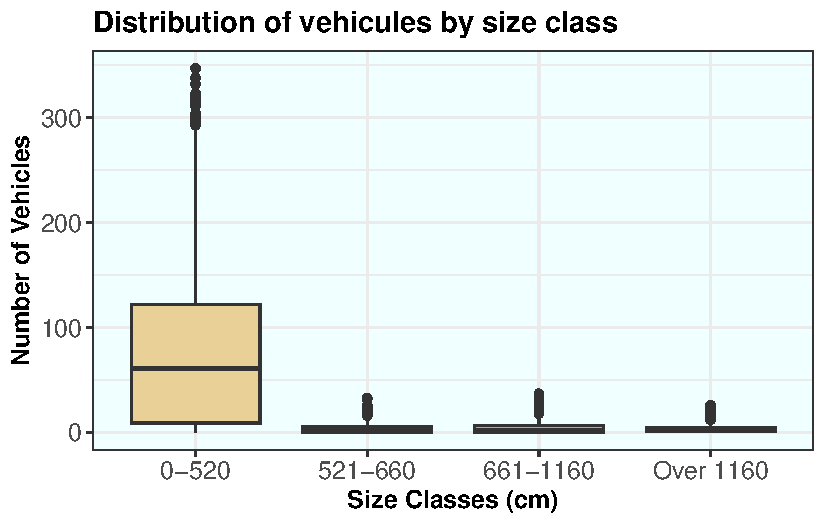
\includegraphics[keepaspectratio]{Tidy_tuesday_6_files/figure-pdf/Showing size class distribution-1.pdf}}

\begin{Shaded}
\begin{Highlighting}[]
\NormalTok{speed }
\end{Highlighting}
\end{Shaded}

\pandocbounded{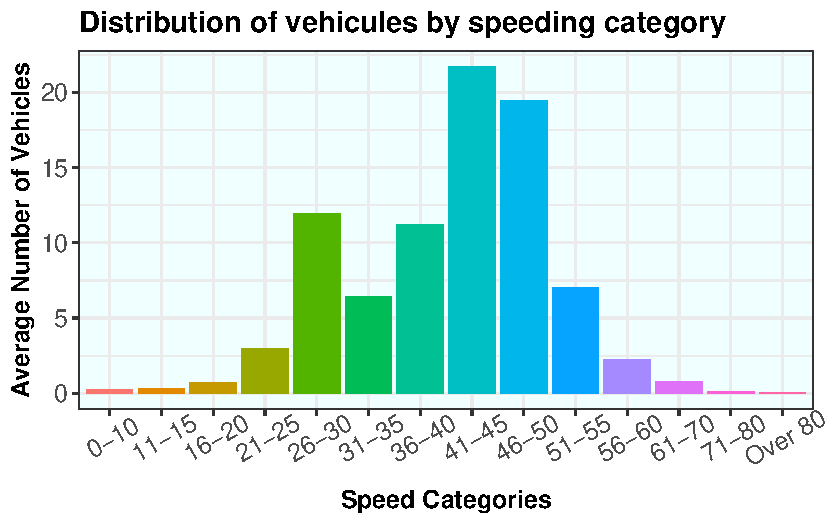
\includegraphics[keepaspectratio]{Tidy_tuesday_6_files/figure-pdf/Showing speed category distribution-1.pdf}}

\section{Discussion}\label{discussion}

\section{Conclusion}\label{conclusion}

\section{Acknowledgments}\label{acknowledgments}

Cras egestas velit mauris, eu mollis turpis pellentesque sit amet.
Interdum et malesuada fames ac ante ipsum primis in faucibus. Nam id
pretium nisi. Sed ac quam id nisi malesuada congue. Sed interdum aliquet
augue, at pellentesque quam rhoncus vitae.


\nolinenumbers
  \bibliography{bibliography.bib}


\end{document}
